% Created 2023-05-06 Sat 00:13
% Intended LaTeX compiler: pdflatex
\documentclass[11pt]{article}
\usepackage[utf8]{inputenc}
\usepackage[T1]{fontenc}
\usepackage{graphicx}
\usepackage{grffile}
\usepackage{longtable}
\usepackage{wrapfig}
\usepackage{rotating}
\usepackage[normalem]{ulem}
\usepackage{amsmath}
\usepackage{textcomp}
\usepackage{amssymb}
\usepackage{capt-of}
\usepackage{hyperref}
\usepackage{float}
\usepackage{verbatim}
\usepackage{xcolor}
\usepackage{listings,multicol}
\author{Ikechukwu Ofili}
\date{May 5, 2023}
\title{Term Project Report\\\medskip
\large CSE 3442: Embedded Systems I}
\hypersetup{
 pdfauthor={Ikechukwu Ofili},
 pdftitle={Term Project Report},
 pdfkeywords={},
 pdfsubject={},
 pdfcreator={Emacs 27.1 (Org mode 9.3)}, 
 pdflang={English}}
\begin{document}

\maketitle
\clearpage \tableofcontents \clearpage

\section{Introduction}
\label{sec:org23da146}
  The project is a haptic walking aid for visually impaired. It's job is to give haptic feedback to the user if certain proximity events are triggered. 
For example, if you are about to hit a wall or you are walking up a flight of stairs. The user can configure the walking aid as much as they need even tweaking the intensity of the vibration


\section{Theory of Operation}
\label{sec:org0325ce6}
To get a wholistic approach of the project, I feel we need to first understand the various parts that make up the project.

\begin{figure}[H]
\centering
\includegraphics[width=0.5\textwidth]{./images/board.jpg}
\caption{The Tiva C Series TM4C123GH6PM microcontroller board}
\end{figure}

First, we have the brain of the walking aid, the microcontroller board, \href{https://www.ti.com/product/TM4C123GH6PM}{ \emph{Texas Instruments} TM4C123GH6PM microcontroller}.
This board powers all the hardware, handles the logic for reading the sensors, choosing to turn on the motor or not, saving user config settings, etc.

This project also uses three ultra-sonic distance sensors which are the HC-SR04 sensors (I will link the datasheet \href{https://www.handsontec.com/dataspecs/HC-SR04-Ultrasonic.pdf}{here}). The sensors are connected to the
microcontroller as GPIOs (general-purpose inputs and outputs) 
I use a timer to measure the amount of time that passed between when the sound wave was pulsed and when it bounces back which I can then use to calculate
the distance using the speed of sound. Then, another timer that times is used to store the current distances measured by these sensors to a global variable \texttt{`dist`}
ten times a second. After that, we then turn on (or off) the motor if the specified distance(s) warrants that. 

\begin{figure}[H]
\centering
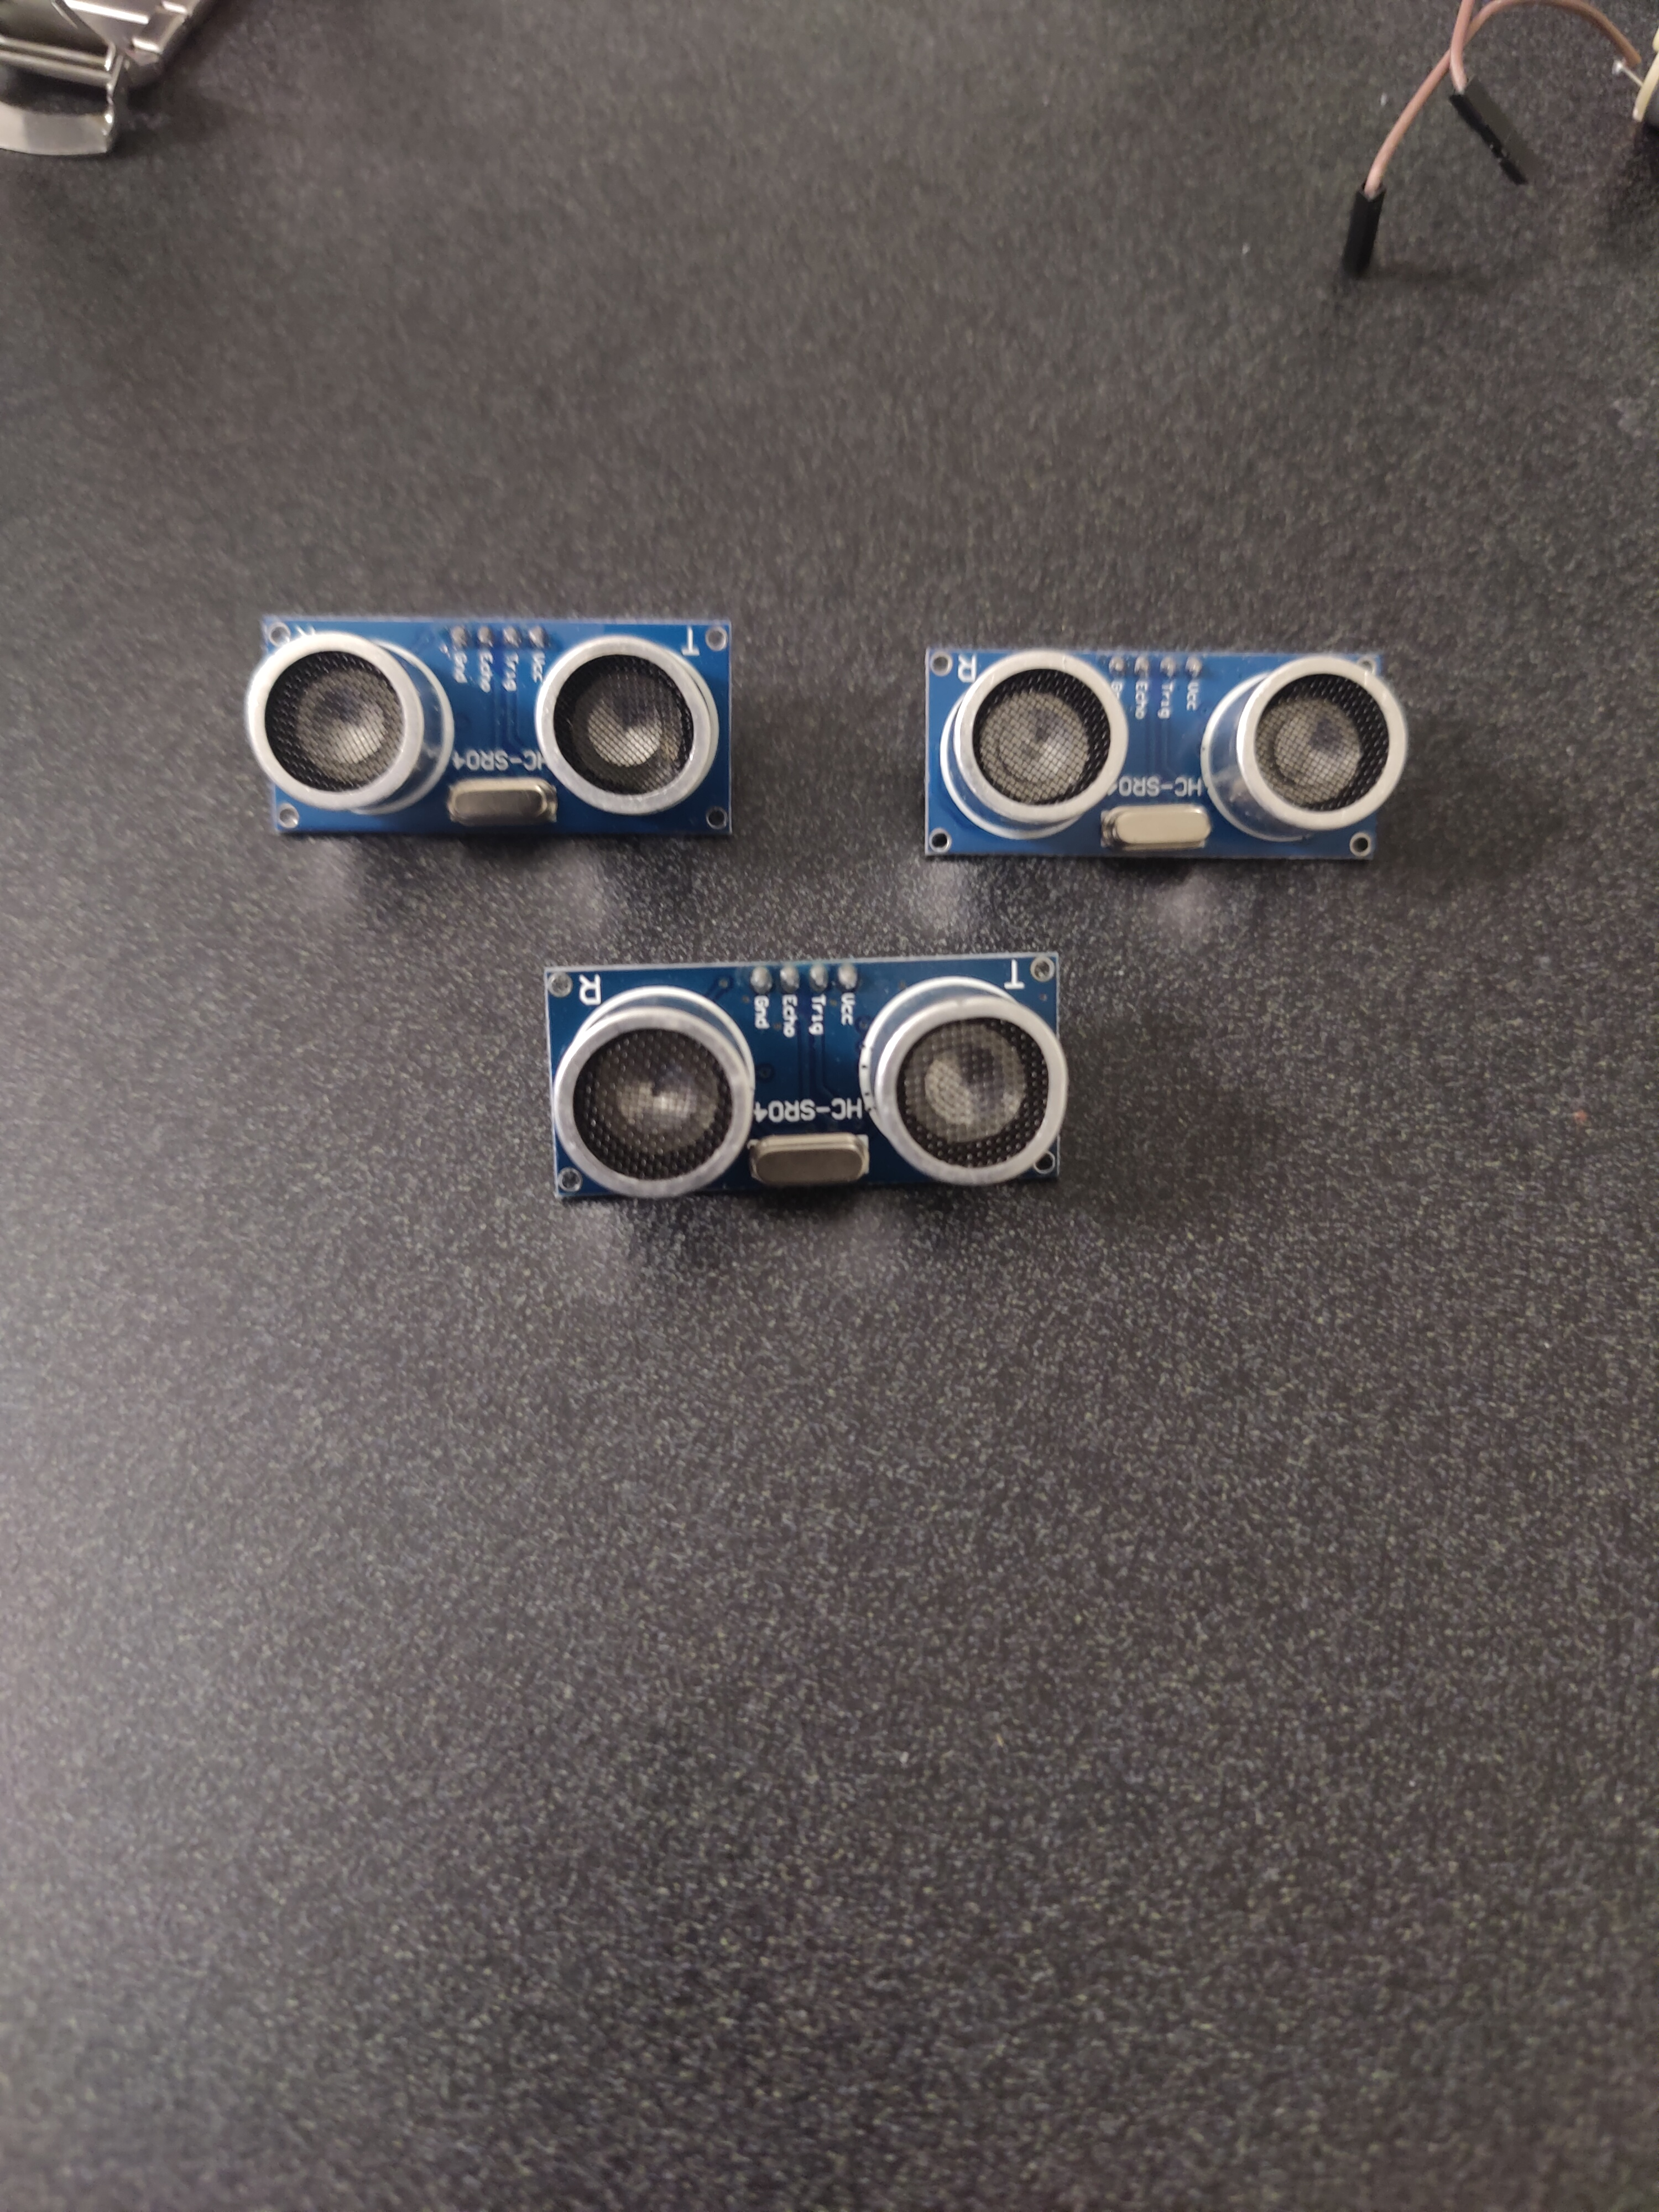
\includegraphics[width=0.7\textwidth]{./images/sensors.jpg}
\caption{HC-SR04 Ultra-sonic sensors}
\end{figure}

The motor used draws a lot of current. Therefore, I could not power it directly using the microcontroller board but I had to use a MOSFET as a switch(ing amplifier)

\begin{figure}[H]
\centering
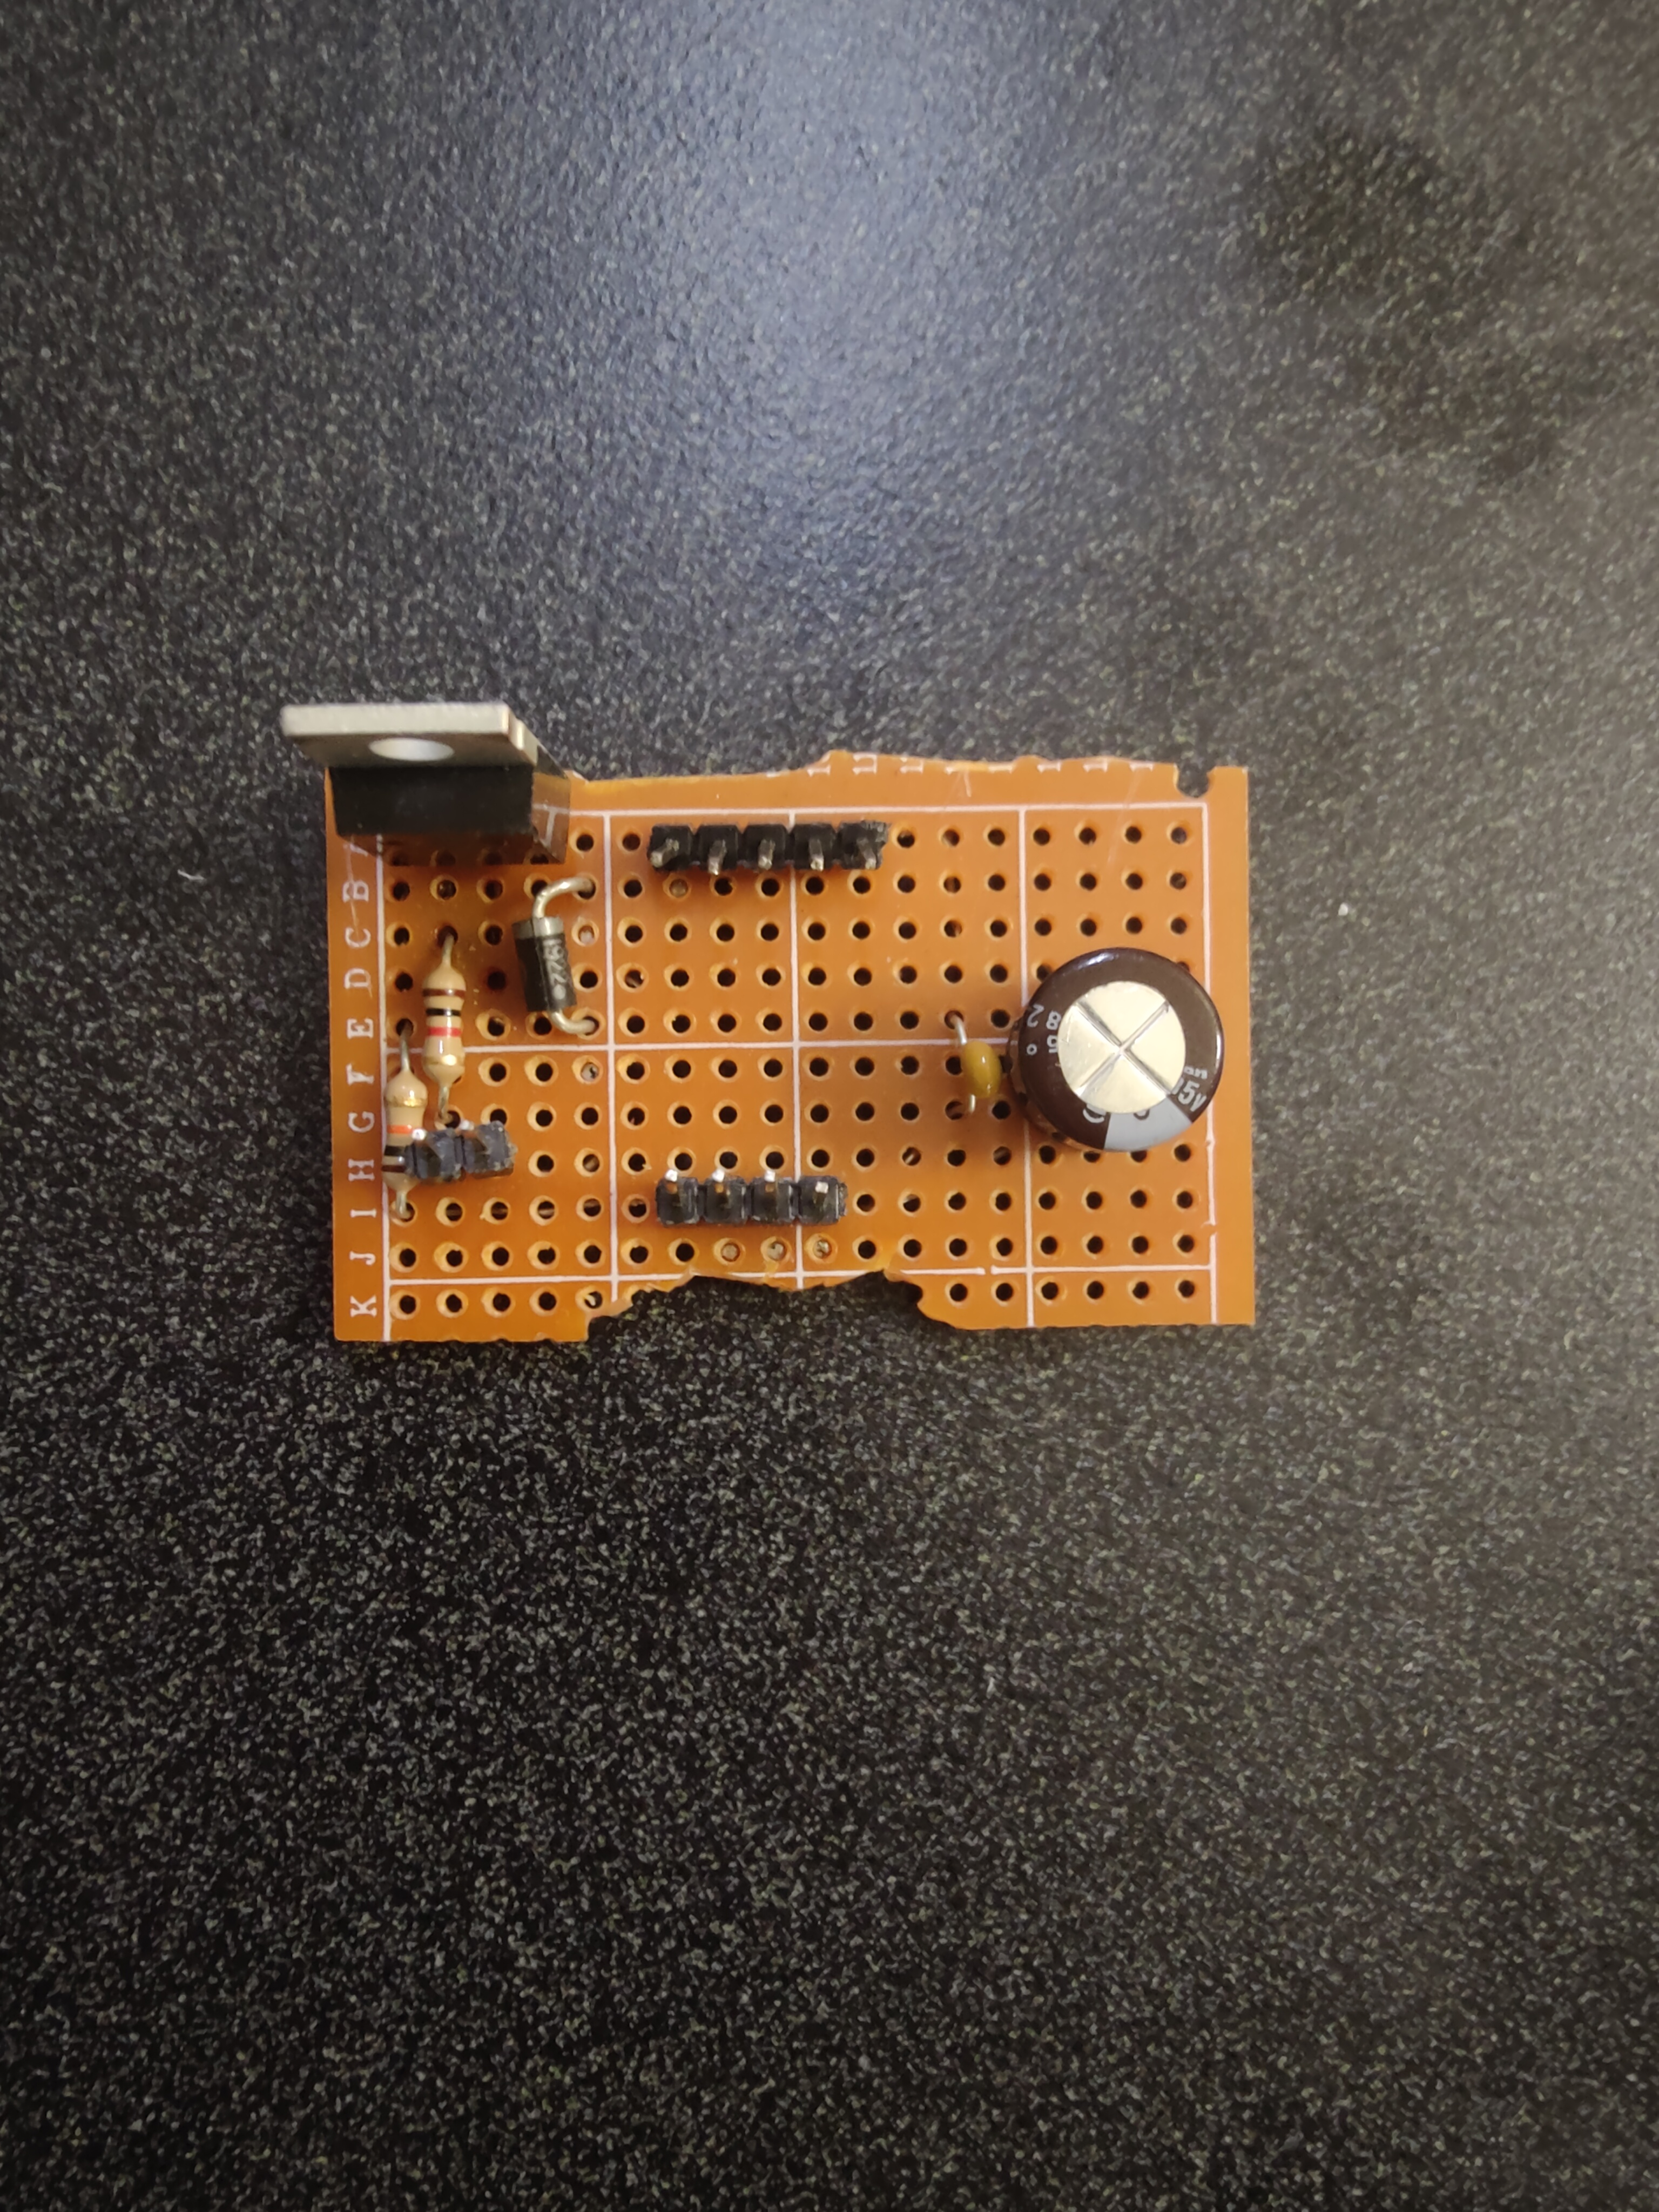
\includegraphics[width=0.7\textwidth]{./images/circuit.jpg}
\caption{Switching circuit for powering the motor}
\end{figure}

A major part of this project is the event system. Users can add certain events that triggers the motors when the event is live. There are 16 simple events and 4 compound ones.
Simple events simply vibrates the cane with a specified pattern when any of the three sensors senses an obstacle between a set distance. A compound event is the conjunction of
two simple events. That is, it sets off when both events are live. The user can also set a specific pattern for those too. An event I used to test the final product and I find
to be very useful is one to detect the next step while climbing up a flight of stairs. The events are also stored to long-term memory so that after power-off, user settings are not lost

\begin{figure}[H]
\centering
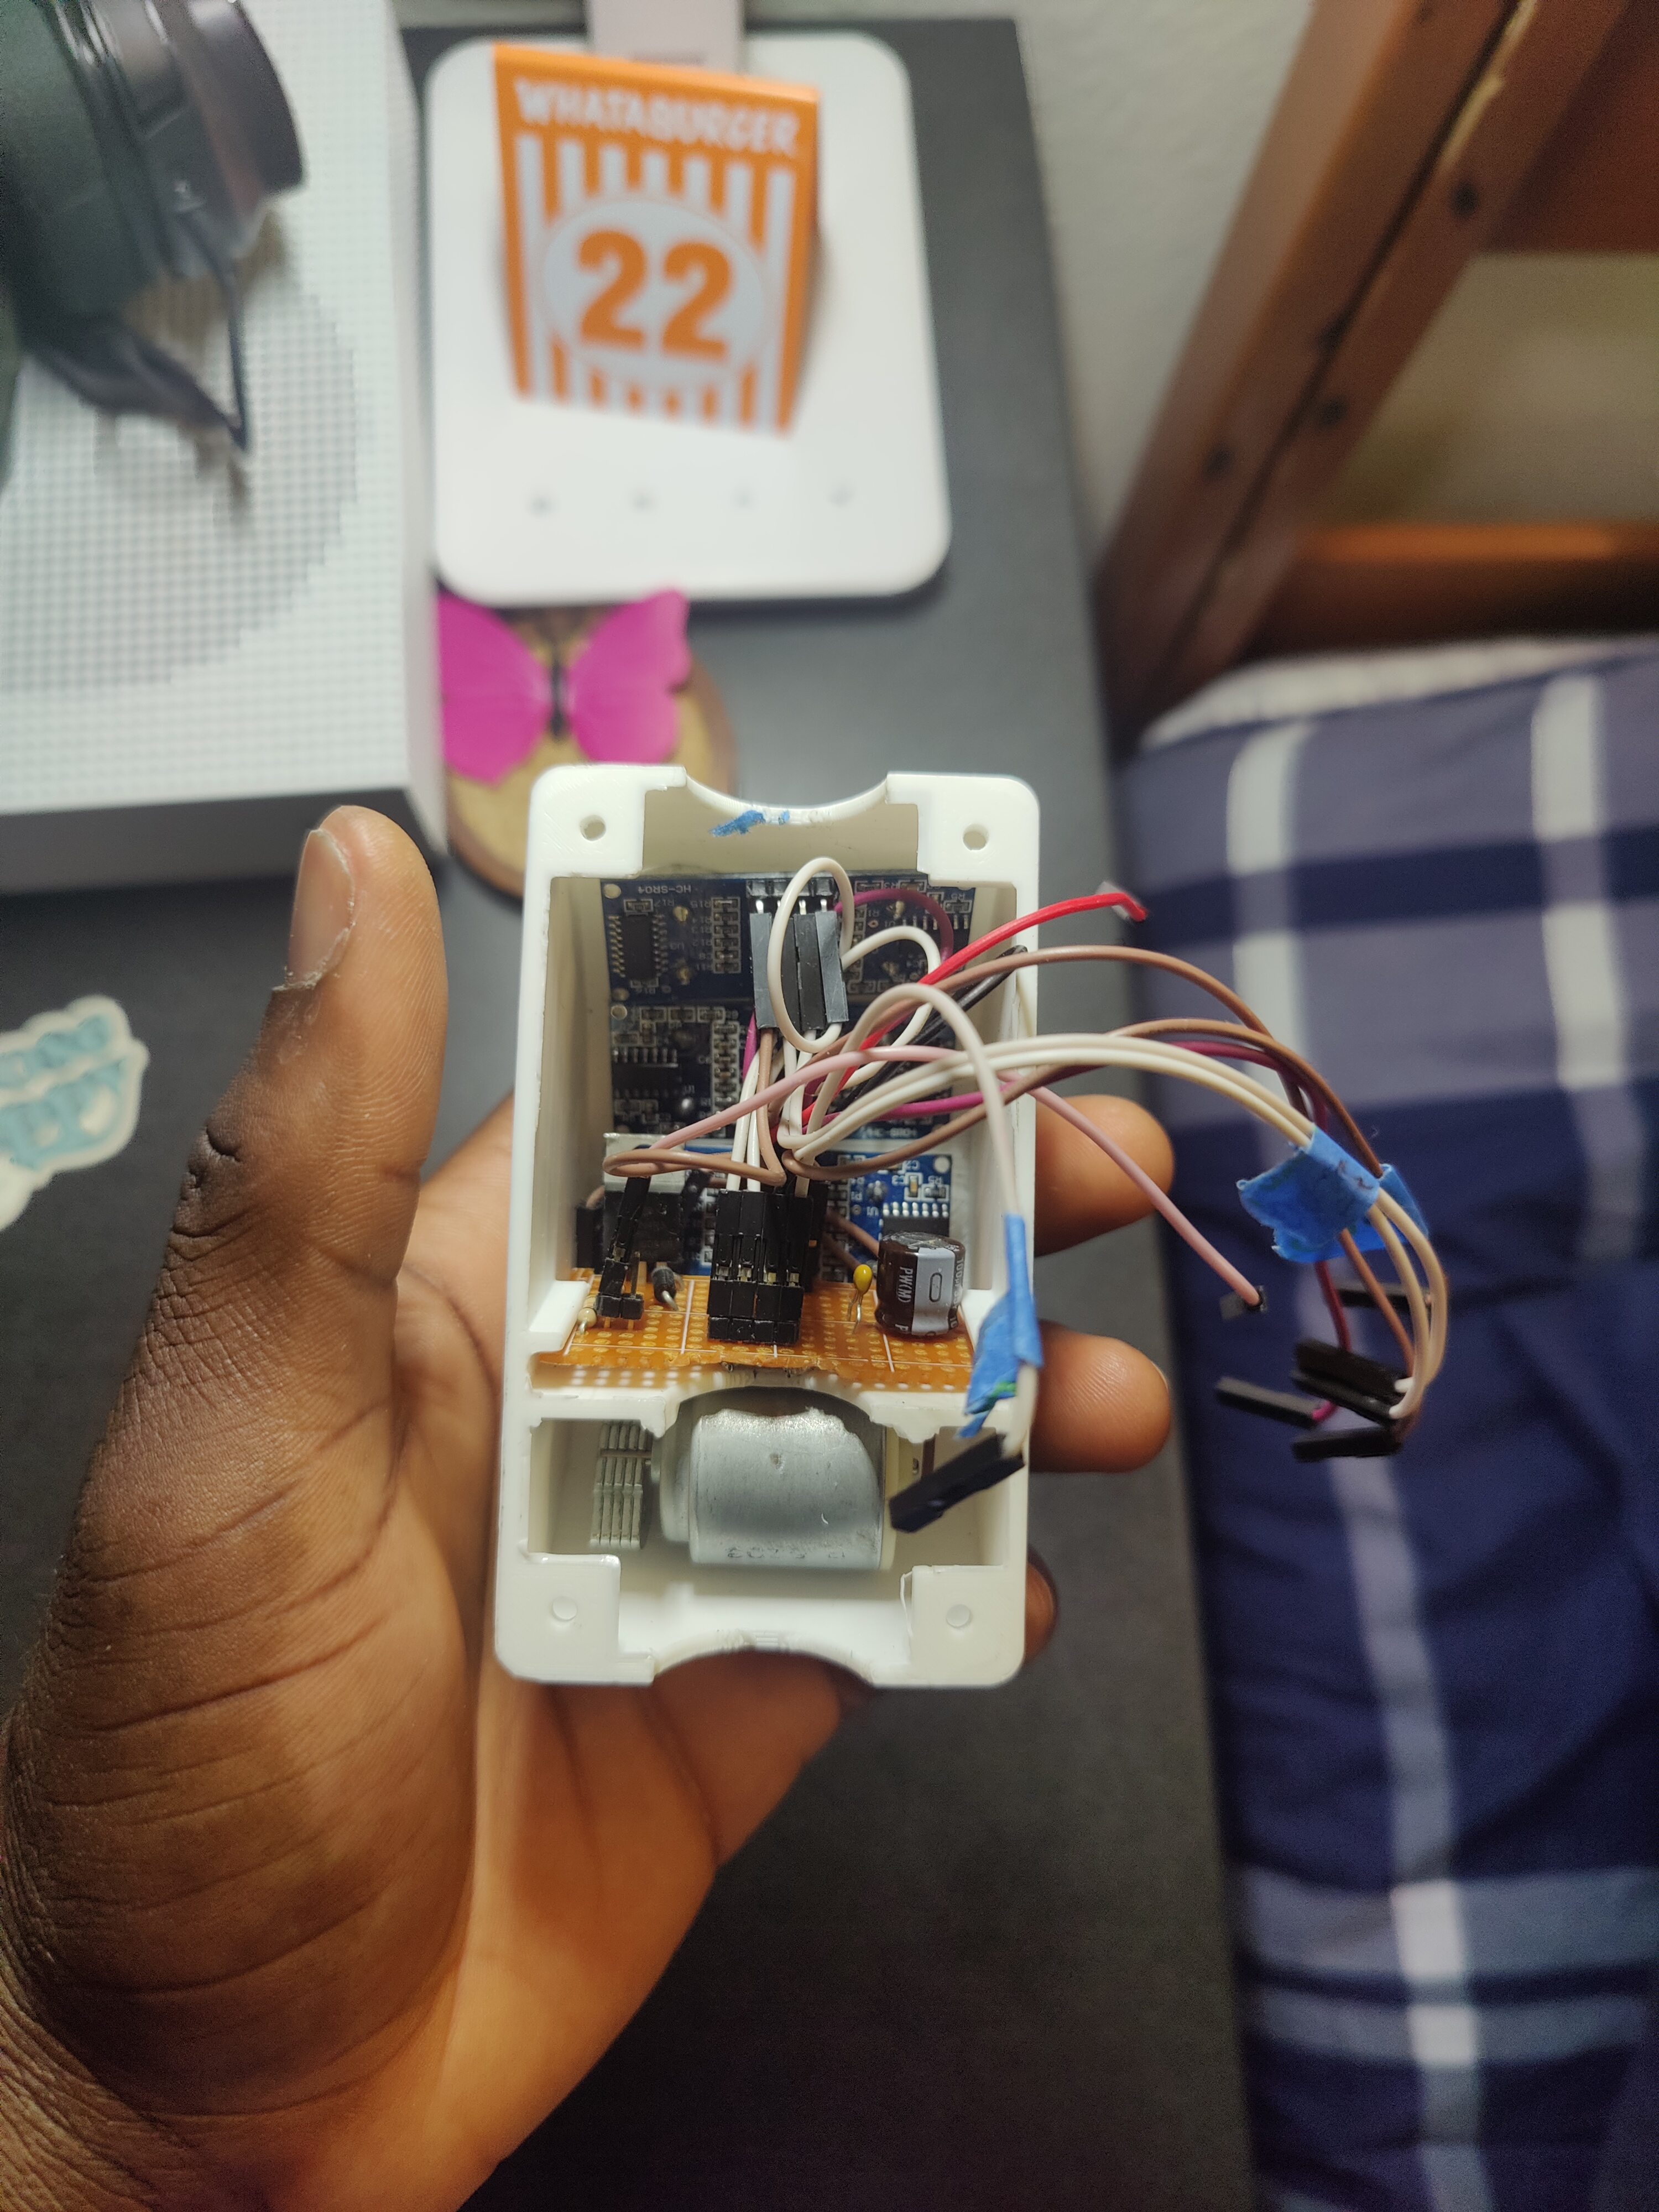
\includegraphics[width=0.5\textwidth]{./images/guts.jpg}
\caption{The sensors, motor and circuit all wired up in the plastic casing}
\end{figure}

\begin{figure}[H]
\centering
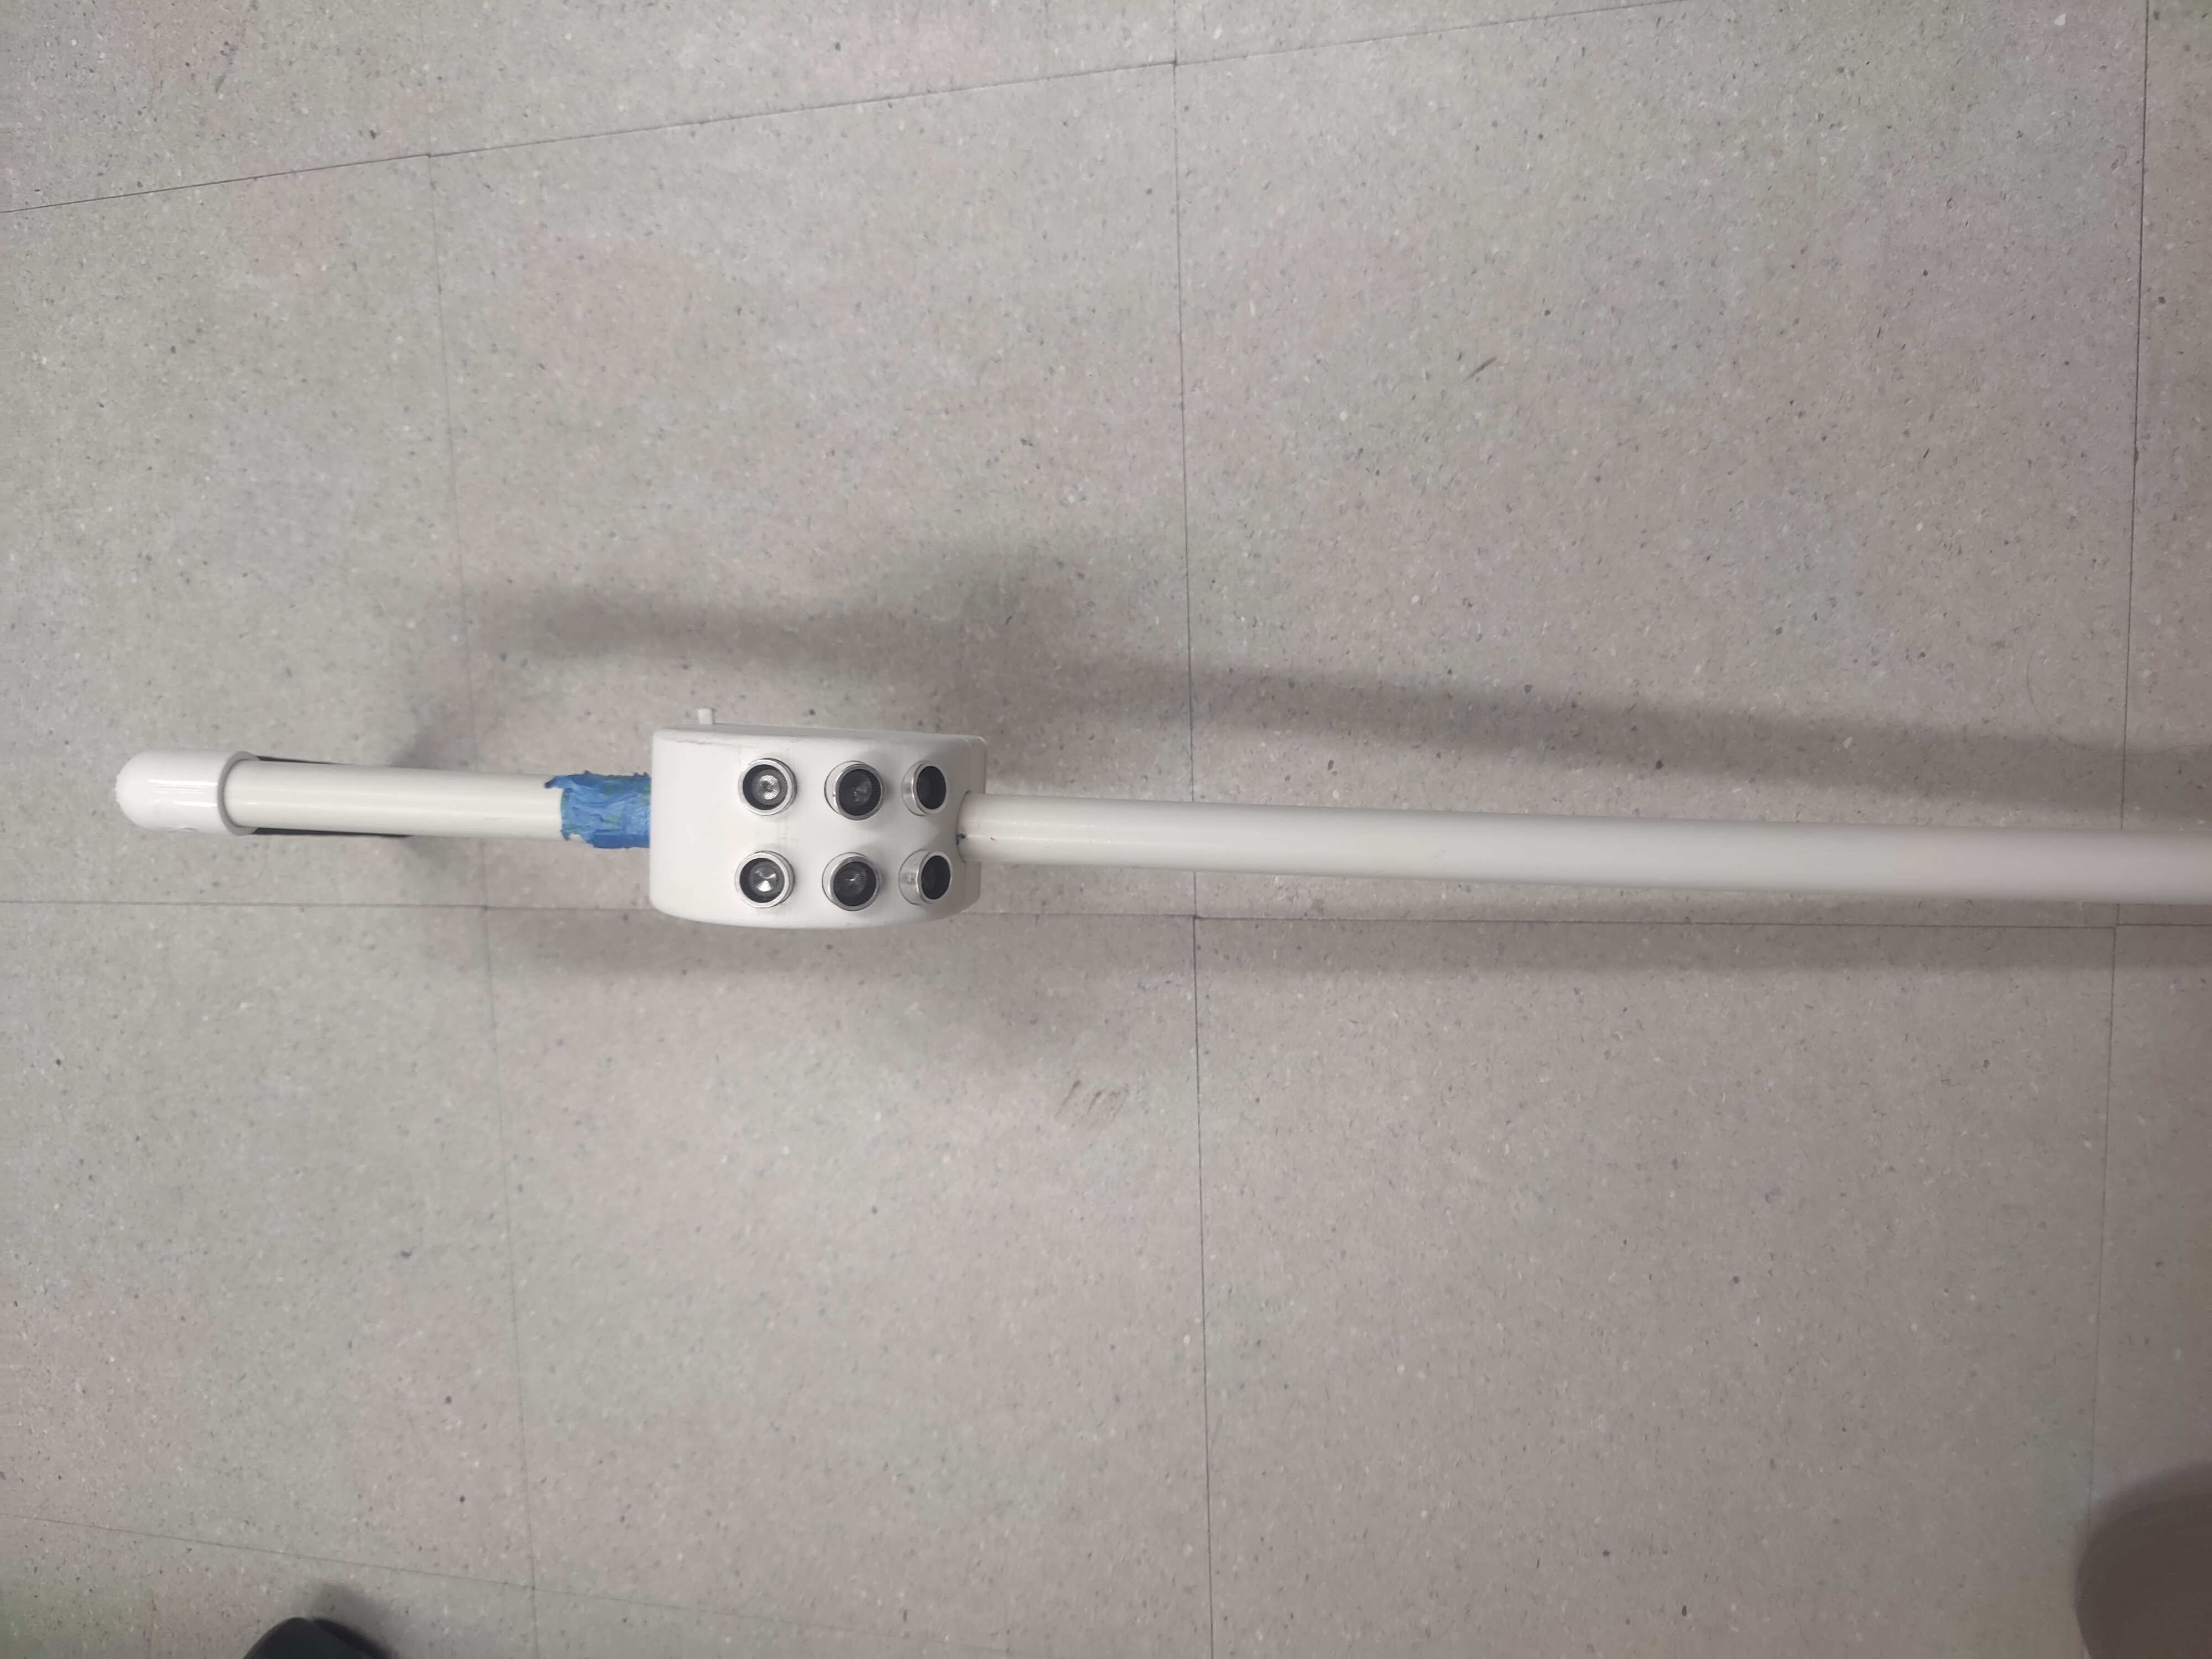
\includegraphics[width=.9\linewidth]{./images/final.jpg}
\caption{A picture of the completed project}
\end{figure} 

Finally, the completed project is housed in a 3D-printed plastic encasing and I used a PVC pipe as a mock-up walking stick for testing. A battery pack is also strapped on for powering
the walking aid outside development.

\section{Code}
\label{sec:orgd0e7caa}
All code for this project was written in C. Development was done in TI's \emph{Code Composer Studio} over a span of about 8 weeks. 
I have included all the files needed to build and run this project in its entirety below.

\clearpage

\lstset{
  language=C,breaklines=true,keywordstyle=\color{blue},
  commentstyle=\color[rgb]{0.13,0.54,0.13},stringstyle=\ttfamily,
  showstringspaces=false
}
  
\lstinputlisting[basicstyle=\tiny]{./EMBEDDEDFINAL/main.c}
%\end{figure*}

\section{Observations}
\label{sec:org99ab552}
The only observations that I noticed while designing and building this project was how unreliable the ultrasonic sensors are. 
Every once in a while, there will be a spike in the readings and some times the readings are wrong altogether if the obstacle is a smoother surface.
However, for our case where we only need a few centimeters of precision, this is fine (as long as the object can reflect the incoming sound waves)
\section{Conclusions}
\label{sec:org50d9f45}
In conclusion, I was able to build a haptic walking aid with user interaction and is actually fairly usable. I learned various embedded systems techniques and concepts along
the way. It was truly a fun and educative project and I cannot wait for more like this
\end{document}
